% ============================================================
% Capítulo 11: Equipe e Colaboração com IA
% ============================================================
\chapter{Equipe e Colaboração com IA}

\section{Introdução}

Software é um esporte coletivo. Nenhum grande sistema foi construído por uma
pessoa sozinha --- nem o Linux, nem o Google, nem o sistema legado de 15 anos
que sustenta sua empresa. A ilusão do gênio solitário é perigosa: ela desvaloriza
comunicação, ignora coordenação e subestima o fator humano que determina se um
projeto vive ou morre.

\begin{itemize}
    \item \textbf{A Lei de Conway}: organizações que projetam sistemas estão
    fadadas a produzir designs que são cópias das estruturas de comunicação
    dessas organizações. Se seus times não se falam, seus microserviços
    também não vão se integrar bem.
    \item \textbf{Consequência prática}: antes de redesenhar a arquitetura,
    redesenhe a organização. Ou pelo menos entenda que uma coisa espelha a
    outra.
    \item \textbf{Software como artefato social}: código é a cristalização de
    decisões humanas. Cada \texttt{if} reflete uma conversa que aconteceu (ou
    que deveria ter acontecido).
    \item \textbf{IA como novo membro do time}: ferramentas de IA mudam a
    dinâmica de equipes. Um engenheiro com IA produz o equivalente a dois ou
    três sem ela --- mas isso muda o tamanho ideal dos times, os rituais, a
    divisão de trabalho.
    \item \textbf{O paradoxo da produtividade}: mais produtividade individual
    exige \textbf{mais} coordenação, não menos. Se cada pessoa produz mais
    código, a superfície de integração cresce proporcionalmente.
\end{itemize}

Este capítulo trata do aspecto mais subestimado da engenharia de software: as
pessoas. Ferramentas mudam, linguagens evoluem, frameworks nascem e morrem.
Mas a capacidade de trabalhar bem em equipe é perene.

% ============================================================
\section{Estruturas de Equipe}

A forma como você organiza seus times determina a forma do software que eles
constroem. Não é metáfora --- é a Lei de Conway em ação.

\subsection{Team Topologies}

O modelo de Team Topologies, proposto por Matthew Skelton e Manuel Pais, define
quatro tipos fundamentais de equipe:

\begin{table}[htbp]
\centering
\caption{Team Topologies: Tipos e Responsabilidades}
\begin{tabular}{|p{3.5cm}|p{4.5cm}|p{5cm}|}
\hline
\textbf{Tipo de Equipe} & \textbf{Responsabilidade} & \textbf{Exemplo} \\
\hline
Stream-Aligned & Entrega contínua de valor em um fluxo de negócio & Equipe de Checkout, Equipe de Onboarding \\
\hline
Platform & Fornece serviços internos que reduzem carga cognitiva dos times de stream & Equipe de Infra, Equipe de CI/CD \\
\hline
Complicated Subsystem & Domina um subsistema que requer conhecimento especializado & Equipe de ML/IA, Equipe de Motor de Regras \\
\hline
Enabling & Ajuda outros times a adotar novas práticas e superar obstáculos & Equipe de DevEx, Equipe de Arquitetura \\
\hline
\end{tabular}
\end{table}

\begin{figure}[htbp]
    \centering
    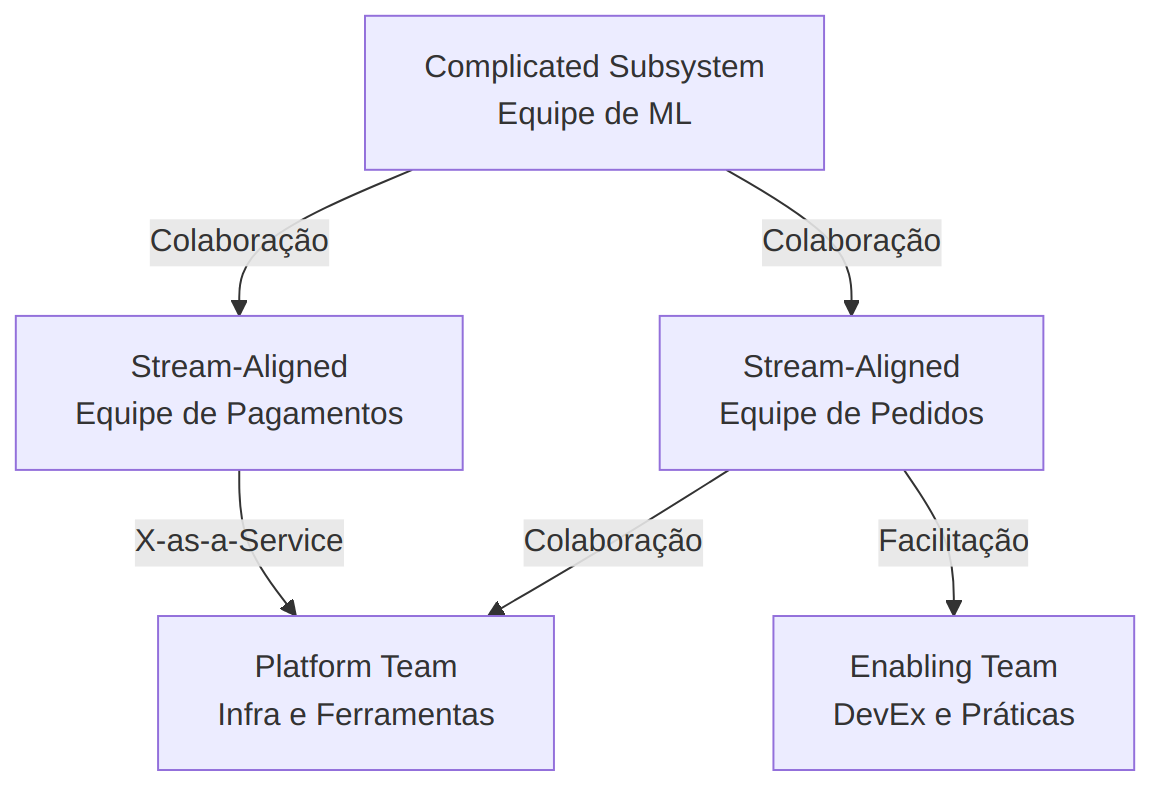
\includegraphics[width=0.85\textwidth]{imagens/11-equipe-colaboracao-ia-01-team-topologies-tipos-de-equipe-e-interacoes.png}
    \caption{Team Topologies -- Tipos de Equipe e Interações}
\end{figure}

\begin{itemize}
    \item \textbf{Stream-Aligned Teams}: são a unidade principal. Cada time é
    dono de ponta a ponta de um fluxo de valor do negócio. Desde o design até
    a operação em produção. Autonomia máxima, dependência mínima.
    \item \textbf{Platform Teams}: existem para que os times de stream não
    precisem reinventar infraestrutura. Oferecem APIs internas, ferramentas,
    pipelines. O produto deles é a plataforma interna.
    \item \textbf{Complicated Subsystem Teams}: quando um componente exige
    conhecimento profundo (criptografia, machine learning, motores de cálculo),
    faz sentido isolá-lo em um time especialista.
    \item \textbf{Enabling Teams}: são temporários por natureza. Ajudam outros
    times a adotar uma prática (observabilidade, testes, IA) e depois saem.
    Não criam dependência permanente.
\end{itemize}

\subsection{Modos de Interação}

\begin{table}[htbp]
\centering
\caption{Modos de Interação entre Times}
\begin{tabular}{|p{3cm}|p{5cm}|p{5cm}|}
\hline
\textbf{Modo} & \textbf{Descrição} & \textbf{Quando Usar} \\
\hline
Colaboração & Dois times trabalham juntos em um problema & Descoberta, inovação, integrações novas \\
\hline
X-as-a-Service & Um time consome a API/serviço do outro & Interfaces estáveis, responsabilidades claras \\
\hline
Facilitação & Um time ajuda outro a desenvolver capacidades & Adoção de novas práticas, remoção de obstáculos \\
\hline
\end{tabular}
\end{table}

\subsection{Equipes Cross-Funcionais e Two-Pizza Teams}

\begin{itemize}
    \item \textbf{Cross-funcional}: o time tem todas as competências necessárias
    para entregar valor sem depender de outro time. Back-end, front-end, QA,
    design, dados --- todos na mesma equipe.
    \item \textbf{Two-pizza teams (Amazon)}: se duas pizzas não alimentam o time,
    ele é grande demais. Na prática, 5 a 8 pessoas. Times menores comunicam-se
    melhor, decidem mais rápido, têm menos overhead de coordenação.
    \item \textbf{Dunbar e software}: o número de canais de comunicação cresce
    com $n(n-1)/2$. Com 5 pessoas são 10 canais. Com 10 pessoas são 45. Com
    20 são 190. Cada canal é uma oportunidade para mal-entendido.
\end{itemize}

\subsection{Manobra Inversa de Conway}

\begin{itemize}
    \item \textbf{O conceito}: se a Lei de Conway diz que o sistema espelha a
    organização, então \textbf{reorganize a organização para produzir a
    arquitetura desejada}.
    \item \textbf{Exemplo}: se você quer microserviços independentes, crie times
    independentes. Se quer um monolito coeso, mantenha um time coeso.
    \item \textbf{Armadilha}: reorganizar sem mudar incentivos, processos e
    cultura não funciona. A estrutura formal muda no organograma; a informal
    continua nos corredores.
\end{itemize}

\subsection{Como a IA Afeta Tamanho e Estrutura de Times}

\begin{itemize}
    \item \textbf{Times menores, mesma entrega}: com IA auxiliando cada membro,
    um time de 4 pode ter a produtividade de um time de 7. Isso é bom --- menos
    overhead de comunicação.
    \item \textbf{Enabling Teams de IA}: um time que ajuda os demais a usar IA
    de forma efetiva é um investimento com retorno exponencial.
    \item \textbf{Novos papéis}: prompt engineer, AI reviewer, curador de
    contexto para LLMs --- funções que não existiam há dois anos.
    \item \textbf{Risco}: times tão pequenos que não têm redundância. Se uma
    pessoa sai, leva metade do conhecimento. O bus factor continua relevante.
\end{itemize}

% ============================================================
\section{Comunicação Técnica Efetiva}

Código é comunicação. Mas não é a única forma. Engenheiros que sabem escrever,
apresentar e documentar decisões multiplicam seu impacto.

\subsection{RFCs e Design Docs}

RFC (Request for Comments) é o documento mais importante que um engenheiro pode
escrever. Ele força clareza de pensamento antes de escrever código.

\begin{table}[htbp]
\centering
\caption{RFC Template Completo}
\begin{tabular}{|p{3.5cm}|p{9.5cm}|}
\hline
\textbf{Seção} & \textbf{Conteúdo} \\
\hline
Título e Autor & Nome descritivo, autor(es), data, status (rascunho/em revisão/aprovado) \\
\hline
Contexto & Por que este documento existe. Qual problema estamos resolvendo. \\
\hline
Proposta & A solução proposta, com detalhes suficientes para implementar. \\
\hline
Alternativas Consideradas & O que mais foi avaliado e por que foi descartado. \\
\hline
Trade-offs & O que ganhamos e o que perdemos com essa decisão. \\
\hline
Impacto & Quais times, serviços e processos são afetados. \\
\hline
Plano de Implementação & Fases, milestones, estimativas de esforço. \\
\hline
Métricas de Sucesso & Como saberemos que funcionou. \\
\hline
Riscos e Mitigações & O que pode dar errado e como reagiremos. \\
\hline
Referências & Links para documentos, artigos, PRs relevantes. \\
\hline
\end{tabular}
\end{table}

\begin{lstlisting}[language={}, caption={Template de RFC em Markdown}]
# RFC: [Titulo Descritivo]

**Autor(es):** [Nome(s)]
**Data:** [YYYY-MM-DD]
**Status:** Rascunho | Em Revisao | Aprovado | Implementado

## Contexto
Por que este documento existe? Qual problema estamos resolvendo?
Qual e o impacto de NAO resolver?

## Proposta
Descricao detalhada da solucao proposta.
Diagramas, exemplos de API, modelos de dados.

## Alternativas Consideradas
| Alternativa | Pros | Contras | Por que descartada |
|-------------|------|---------|-------------------|
| Opcao A     | ...  | ...     | ...               |
| Opcao B     | ...  | ...     | ...               |

## Trade-offs
- Ganhamos: [X, Y, Z]
- Perdemos: [A, B, C]
- Divida tecnica introduzida: [se houver]

## Plano de Implementacao
1. Fase 1: [descricao] - [estimativa]
2. Fase 2: [descricao] - [estimativa]

## Metricas de Sucesso
- [ ] Metrica 1: [definicao, baseline, meta]
- [ ] Metrica 2: [definicao, baseline, meta]

## Riscos
| Risco | Probabilidade | Impacto | Mitigacao |
|-------|--------------|---------|-----------|
| ...   | Alta/Media   | Alto    | ...       |
\end{lstlisting}

\begin{itemize}
    \item \textbf{Quando escrever uma RFC}: qualquer mudança que afete mais de
    um time, que leve mais de uma semana para implementar ou que seja
    irreversível.
    \item \textbf{O valor está no processo}: o documento final é secundário. O
    valor está nas conversas que ele provoca e nas alternativas que ele força
    a considerar.
    \item \textbf{Revisão assíncrona}: RFCs permitem que pessoas em fusos
    horários diferentes contribuam. Cada comentário é registrado, cada
    decisão é rastreável.
\end{itemize}

\subsection{Documentação de Decisões}

\begin{itemize}
    \item \textbf{Architecture Decision Records (ADRs)}: documentos curtos que
    registram decisões técnicas importantes. Título, contexto, decisão,
    consequências. Michael Nygard formalizou o formato.
    \item \textbf{Por que documentar decisões}: daqui a seis meses, alguém
    (talvez você mesmo) vai perguntar ``por que fizemos assim?''. O ADR
    responde sem precisar de arqueologia em commits.
    \item \textbf{Decisões são contextuais}: uma boa decisão em 2023 pode ser
    ruim em 2025. O ADR registra o contexto da época, evitando julgamentos
    retroativos injustos.
\end{itemize}

\subsection{Comunicação Assíncrona vs. Síncrona}

\begin{figure}[htbp]
    \centering
    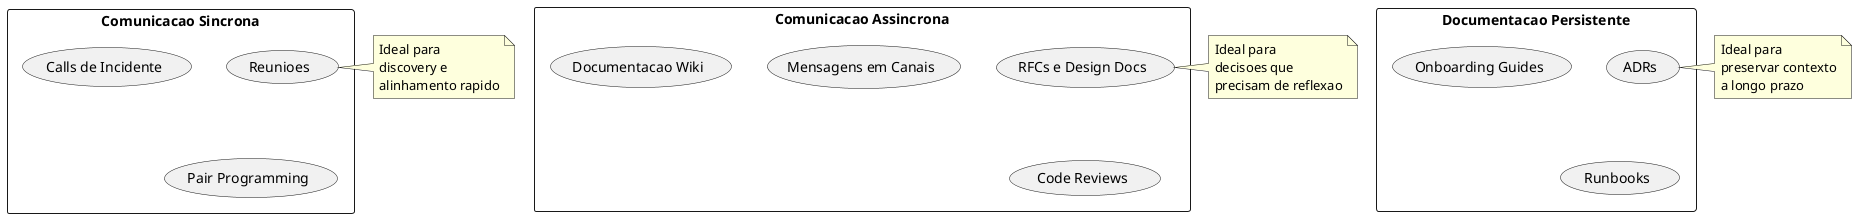
\includegraphics[width=0.85\textwidth]{imagens/11-equipe-colaboracao-ia-02-padroes-de-comunicacao-em-equipes-de-engenharia.png}
    \caption{Padrões de Comunicação em Equipes de Engenharia}
\end{figure}

\begin{itemize}
    \item \textbf{Regra de ouro}: use síncrono para descobrir, assíncrono para
    decidir, documentação para preservar.
    \item \textbf{Reuniões que deveriam ser documentos}: se a reunião é apenas
    para transmitir informação, escreva um documento. Reuniões são para
    \textbf{interação}, não \textbf{transmissão}.
    \item \textbf{Documentos que deveriam ser reuniões}: se o assunto é ambíguo,
    emocional ou tem muitas partes interessadas com opiniões divergentes,
    converse antes de escrever.
\end{itemize}

\subsection{Escrita como Superpoder}

\begin{itemize}
    \item \textbf{Engenheiros que escrevem bem lideram}: Jeff Bezos proibiu
    PowerPoints na Amazon. Narrativas de 6 páginas substituem slides. Escrever
    força clareza.
    \item \textbf{Escrita técnica efetiva}: frases curtas, voz ativa, exemplos
    concretos, estrutura lógica. Se o leitor precisa reler, o autor falhou.
    \item \textbf{IA como assistente de escrita}: use LLMs para revisar clareza,
    sugerir estrutura, identificar ambiguidades. Mas o pensamento original é
    seu --- a IA polui, você refina.
    \item \textbf{Feedback técnico construtivo}: critique a ideia, não a pessoa.
    ``Essa abordagem pode ter problemas de escala porque...'' em vez de ``isso
    está errado''.
\end{itemize}

% ============================================================
\section{Mentoria e Crescimento}

Times fortes são feitos de pessoas que crescem. Se ninguém evolui, o time
estagna --- e estagnar em tecnologia é retroceder.

\subsection{Pair Programming}

Pair programming não é duas pessoas no mesmo teclado. É uma técnica
estruturada com variações para diferentes situações.

\begin{table}[htbp]
\centering
\caption{Pair Programming: Estilos e Quando Usar}
\begin{tabular}{|p{3cm}|p{4.5cm}|p{5.5cm}|}
\hline
\textbf{Estilo} & \textbf{Como Funciona} & \textbf{Quando Usar} \\
\hline
Driver/Navigator & Um digita, outro dirige estrategicamente. O navigator pensa no panorama enquanto o driver implementa. & Tarefas que exigem atenção a detalhes e visão estratégica simultaneamente. \\
\hline
Ping-Pong & Um escreve o teste, outro faz passar. Alternam a cada ciclo. Combina TDD com pair. & Lógica de negócio bem definida, desenvolvimento orientado a testes. \\
\hline
Strong Style & ``Para uma ideia ir da sua cabeça para o computador, ela precisa passar pelas mãos do outro.'' & Transferência de conhecimento, mentoria ativa, problemas exploratórios. \\
\hline
Mob Programming & Todo o time em um problema, um teclado. Rotação a cada poucos minutos. & Problemas de design difíceis, onboarding de novo membro, decisões arquiteturais. \\
\hline
\end{tabular}
\end{table}

\begin{itemize}
    \item \textbf{Pair com IA}: a IA assume o papel de navigator ou de rubber
    duck sofisticado. Você dirige, ela sugere. Funciona surpreendentemente bem
    para exploração de problemas novos.
    \item \textbf{Quando não fazer pair}: tarefas mecânicas que não exigem
    julgamento, refatorações triviais, trabalho que precisa de foco profundo
    individual.
    \item \textbf{O custo do pair}: duas pessoas, uma tarefa. Parece desperdício.
    Mas a redução de bugs, a transferência de conhecimento e a qualidade do
    design compensam. Pesquisas mostram que pair programming reduz defeitos
    em 15\% a 60\%.
\end{itemize}

\subsection{Mentoria Reversa}

\begin{itemize}
    \item \textbf{O conceito}: juniores mentoram seniores. Sim, ao contrário.
    Juniores trazem perspectivas frescas, conhecimento de ferramentas novas,
    questionamentos que seniores já pararam de fazer.
    \item \textbf{Exemplo}: um júnior ensina o sênior a usar Copilot de forma
    efetiva. O sênior ensina o júnior a avaliar criticamente o que o Copilot
    sugere. Ambos crescem.
    \item \textbf{Benefício oculto}: mentoria reversa destrói hierarquias
    artificiais e cria uma cultura onde perguntar ``não sei'' é normal,
    independentemente do nível.
\end{itemize}

\subsection{Code Reviews como Aprendizado}

\begin{itemize}
    \item \textbf{Objetivo primário}: aprendizado e disseminação de
    conhecimento. Pegar bugs é bônus --- testes fazem isso melhor.
    \item \textbf{O que revisar}: design, clareza, nomes, abstrações,
    testabilidade. Não perca tempo com formatação --- linters fazem isso.
    \item \textbf{Como dar feedback}: seja específico, explique o porquê,
    ofereça alternativas. ``Considere extrair essa lógica para um serviço
    separado porque ela é usada em 3 contextos diferentes'' é melhor que
    ``refatore isso''.
    \item \textbf{IA como primeiro revisor}: use IA para uma primeira passada
    automatizada (estilo, padrões, bugs óbvios). O revisor humano foca em
    design e lógica de negócio.
\end{itemize}

\subsection{IA como Tutor Personalizado}

\begin{itemize}
    \item \textbf{Aprendizado sob demanda}: ``explique o padrão CQRS como se
    eu fosse um engenheiro pleno que nunca trabalhou com event sourcing''.
    A IA adapta a explicação ao nível e contexto.
    \item \textbf{Exercícios personalizados}: peça à IA para criar exercícios
    baseados no código real do seu projeto. Aprendizado contextualizado é
    mais efetivo.
    \item \textbf{Simulação de entrevistas}: a IA faz perguntas técnicas,
    avalia respostas, sugere melhorias. Prática sem constrangimento.
    \item \textbf{Limitação}: a IA não substitui o feedback humano sobre
    habilidades interpessoais, comunicação e colaboração. Para soft skills,
    mentores humanos continuam insubstituíveis.
\end{itemize}

\subsection{Carreira: IC vs. Management}

\begin{itemize}
    \item \textbf{Individual Contributor (IC)}: profundidade técnica crescente.
    De júnior a staff engineer, principal engineer, distinguished engineer.
    Cada nível exige mais influência sem autoridade direta.
    \item \textbf{Management}: de tech lead a engineering manager, director,
    VP. Cada nível afasta mais do código e aproxima mais de pessoas, processos
    e estratégia.
    \item \textbf{A armadilha}: promover o melhor engenheiro para gerente.
    Excelência técnica não implica excelência em gestão. Ofereça ambos os
    caminhos com remuneração equivalente.
    \item \textbf{T-shaped vs. Pi-shaped}: engenheiros T-shaped têm
    profundidade em uma área e amplitude em várias. Pi-shaped têm
    profundidade em \textbf{duas} áreas. Na era da IA, Pi-shaped (ex.:
    back-end + ML, ou infra + segurança) é cada vez mais valioso.
\end{itemize}

% ============================================================
\section{Gestão de Conhecimento}

Conhecimento que existe apenas na cabeça de uma pessoa não é conhecimento
organizacional --- é risco.

\subsection{Bus Factor}

\begin{itemize}
    \item \textbf{Definição}: o número de pessoas que precisam ser atropeladas
    por um ônibus para o projeto parar. Se a resposta é 1, você tem um
    problema sério.
    \item \textbf{Como melhorar}: pair programming rotativo, documentação de
    decisões, code reviews obrigatórios com rodízio de revisores, sessões de
    knowledge sharing.
    \item \textbf{Métrica prática}: para cada componente crítico, quantas
    pessoas conseguem fazer uma mudança significativa sem ajuda? Se é menos
    de 2, ação imediata necessária.
\end{itemize}

\subsection{Onboarding Eficiente}

Um bom onboarding paga dividendos por toda a permanência do novo membro.

\begin{figure}[htbp]
    \centering
    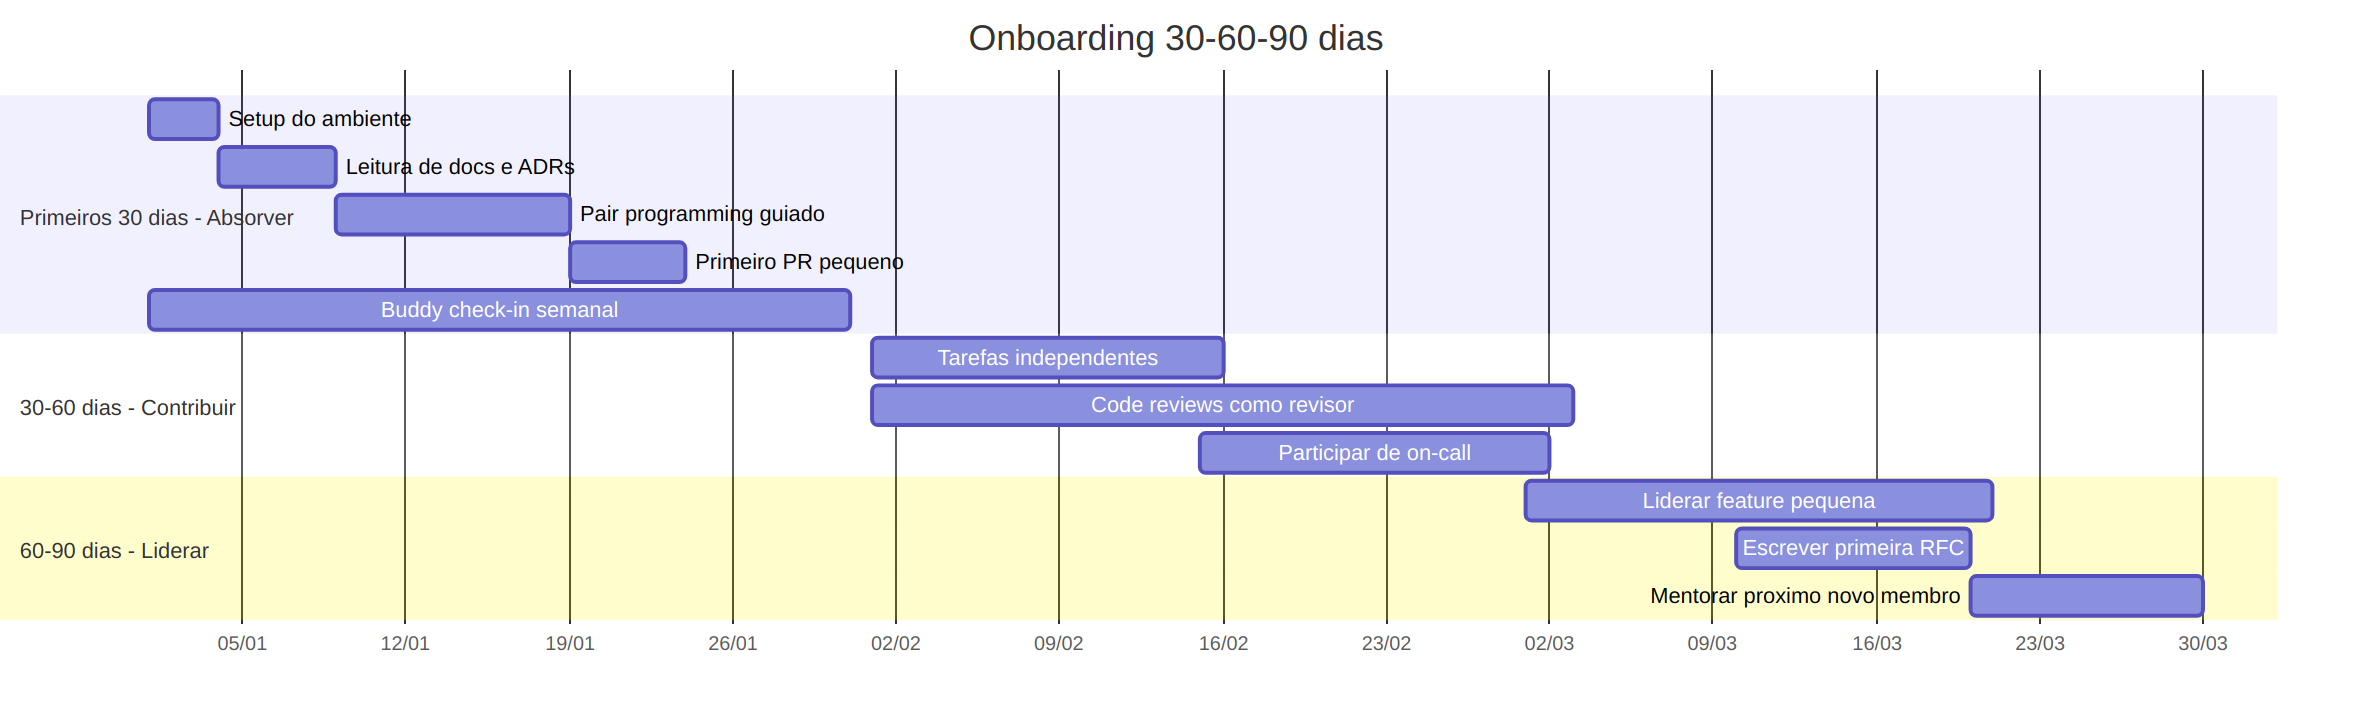
\includegraphics[width=0.85\textwidth]{imagens/11-equipe-colaboracao-ia-03-plano-de-onboarding-30-60-90-dias.png}
    \caption{Plano de Onboarding 30-60-90 dias}
\end{figure}

\begin{lstlisting}[language={}, caption={Template de Plano de Onboarding}]
# Onboarding: [Nome do Novo Membro]

## Buddy: [Nome]
## Data de Inicio: [YYYY-MM-DD]

### Semana 1: Ambiente e Contexto
- [ ] Setup completo do ambiente de desenvolvimento
- [ ] Acesso a todos os repositorios, ferramentas, dashboards
- [ ] Leitura do README principal e ADRs dos ultimos 6 meses
- [ ] Reuniao 1:1 com cada membro do time (30 min cada)
- [ ] Primeira build local funcionando

### Semana 2-4: Absorcao Guiada
- [ ] Pair programming diario com membros diferentes
- [ ] Primeiro PR: bug fix ou melhoria pequena
- [ ] Entender o pipeline de CI/CD
- [ ] Participar de todas as cerimonias do time como observador

### Mes 2: Contribuicao Ativa
- [ ] Assumir tarefas do backlog de forma independente
- [ ] Fazer code reviews (pelo menos 2 por semana)
- [ ] Shadow de on-call por uma semana
- [ ] Feedback 360 informal: como esta a integracao?

### Mes 3: Autonomia
- [ ] Liderar implementacao de uma feature
- [ ] Escrever RFC ou ADR
- [ ] Apresentar algo no show-and-tell
- [ ] Identificar uma melhoria no processo de onboarding
\end{lstlisting}

\subsection{Guildas e Comunidades de Prática}

\begin{itemize}
    \item \textbf{Guildas}: grupos horizontais que cruzam times verticais.
    Guilda de Front-end, Guilda de Segurança, Guilda de Dados. Compartilham
    práticas, padrões e aprendizados.
    \item \textbf{Comunidades de prática}: menos formais que guildas. Pessoas
    interessadas em um tema se reúnem periodicamente para discutir. Sem
    hierarquia, sem obrigação.
    \item \textbf{Tech talks internas (brown bags)}: apresentações curtas
    (30--45 minutos) durante o almoço. Qualquer pessoa pode apresentar.
    Temas: algo que aprendeu, um post-mortem, uma ferramenta nova, uma
    técnica que testou.
    \item \textbf{O valor oculto}: guildas e tech talks criam conexões
    horizontais entre times. Essas conexões informais resolvem problemas
    mais rápido que qualquer processo formal.
\end{itemize}

\subsection{IA como Sistema de Recuperação de Conhecimento}

\begin{itemize}
    \item \textbf{RAG (Retrieval-Augmented Generation)}: conecte um LLM à
    base de conhecimento interna da empresa. Documentação, ADRs, RFCs,
    Slack, wikis. A IA busca e sintetiza em linguagem natural.
    \item \textbf{Exemplo prático}: ``como funciona a autenticação no serviço
    de pagamentos?'' --- a IA busca nos ADRs, no código, na wiki e monta
    uma resposta contextualizada.
    \item \textbf{Cuidados}: dados sensíveis exigem controle de acesso no RAG.
    Nem toda informação deve estar acessível a todos.
    \item \textbf{Manutenção da base}: conhecimento desatualizado é pior que
    conhecimento inexistente. Estabeleça rituais de revisão trimestral da
    documentação.
\end{itemize}

\begin{figure}[htbp]
    \centering
    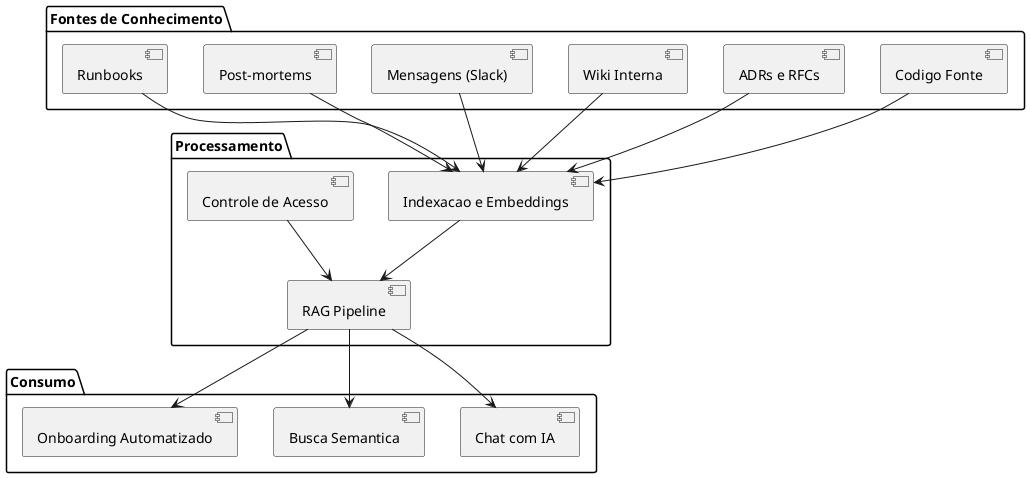
\includegraphics[width=0.85\textwidth]{imagens/11-equipe-colaboracao-ia-04-ecossistema-de-gestao-de-conhecimento.png}
    \caption{Ecossistema de Gestão de Conhecimento}
\end{figure}

% ============================================================
\section{Conflitos Técnicos}

Conflito técnico saudável é sinal de time que pensa. Ausência de conflito
é sinal de time que desistiu.

\subsection{Disagree and Commit}

\begin{itemize}
    \item \textbf{O princípio}: debata vigorosamente, mas quando a decisão for
    tomada, todos se comprometem. Sabotagem passiva (``eu avisei que não ia
    funcionar'') é tóxica.
    \item \textbf{Requisitos}: todos tiveram oportunidade de ser ouvidos. A
    decisão foi transparente. Os critérios foram explícitos.
    \item \textbf{Reversibilidade}: decisões reversíveis (``portas de duas
    mãos'') devem ser tomadas rápido. Decisões irreversíveis (``portas de
    uma mão'') merecem mais debate.
\end{itemize}

\subsection{Consenso vs. Decisão do Tech Lead}

\begin{itemize}
    \item \textbf{Consenso}: todos concordam. Ideal, mas lento. Funciona em
    times pequenos (3--5) e decisões de alto impacto.
    \item \textbf{Consultivo}: o tech lead decide, mas consulta todos antes.
    Bom equilíbrio entre velocidade e inclusão.
    \item \textbf{Autoritário}: o tech lead decide sozinho. Rápido, mas
    perigoso se usado com frequência. Reservado para emergências e impasses.
    \item \textbf{Regra prática}: quanto mais reversível a decisão, menos
    consenso necessário. Quanto mais irreversível, mais consulta.
\end{itemize}

\subsection{Quando Debater vs. Quando Decidir}

\begin{figure}[htbp]
    \centering
    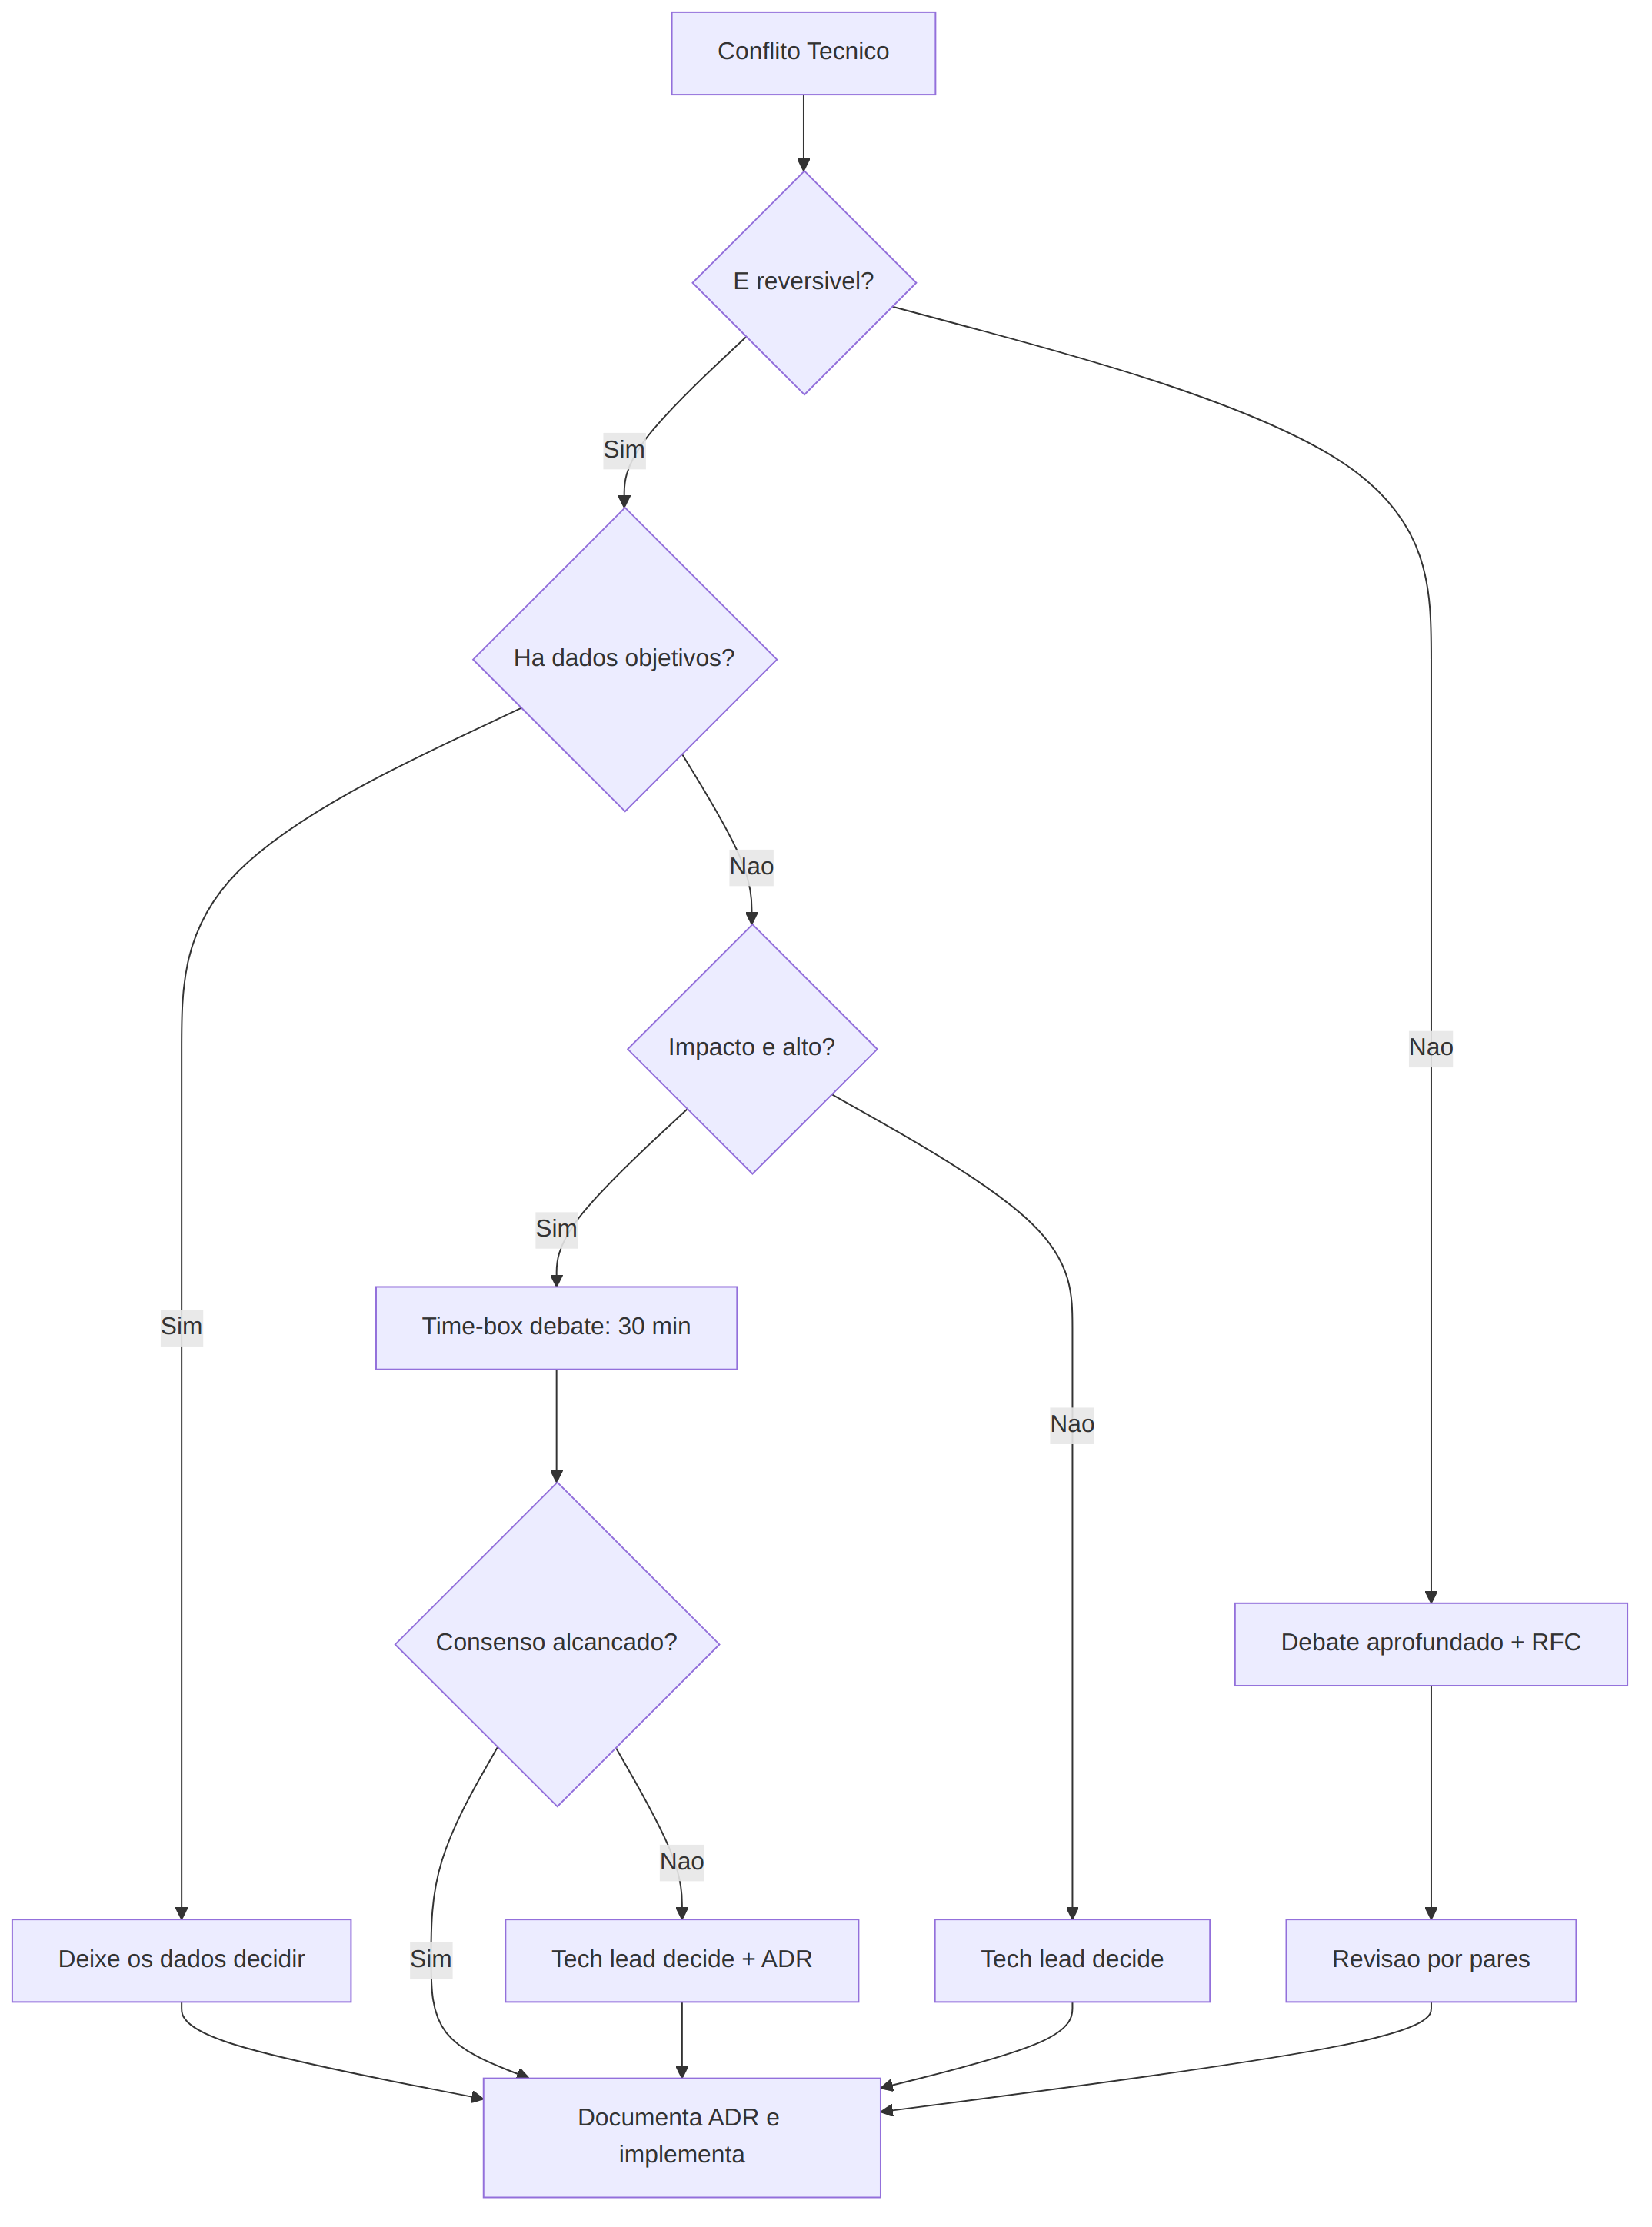
\includegraphics[width=0.85\textwidth]{imagens/11-equipe-colaboracao-ia-05-arvore-de-decisao-para-conflitos-tecnicos.png}
    \caption{Árvore de Decisão para Conflitos Técnicos}
\end{figure}

\subsection{O Papel dos Dados}

\begin{itemize}
    \item \textbf{Benchmarks sobre opiniões}: ``eu acho que o framework X é
    mais rápido'' não vale. ``Nosso benchmark mostra que X processa 3.200
    req/s vs. 2.100 do Y no nosso caso de uso'' vale.
    \item \textbf{Proof of Concept (PoC)}: quando o debate empaca, construa.
    Uma PoC de 2 dias vale mais que 2 semanas de discussão.
    \item \textbf{Métricas de produção}: dados reais de sistemas em produção
    encerram debates teóricos. Latência, error rate, throughput --- números
    não mentem (mas podem ser mal interpretados).
\end{itemize}

\subsection{IA como Mediador Objetivo}

\begin{itemize}
    \item \textbf{Análise imparcial}: ``temos duas propostas arquiteturais.
    Aqui estão os requisitos, as restrições e os trade-offs de cada uma.
    Analise objetivamente.'' A IA não tem ego investido em nenhuma proposta.
    \item \textbf{Pesquisa de precedentes}: ``quais empresas de escala similar
    à nossa adotaram a abordagem A vs. B? Quais foram os resultados
    reportados?''
    \item \textbf{Limitação importante}: a IA não conhece o contexto político,
    cultural e emocional da sua organização. Ela analisa o técnico, não o
    humano.
\end{itemize}

\subsection{Conflito Saudável vs. Conflito Tóxico}

\begin{itemize}
    \item \textbf{Saudável}: foco no problema, respeito mútuo, disposição para
    mudar de ideia diante de evidências, energia direcionada para a melhor
    solução.
    \item \textbf{Tóxico}: ataques pessoais, agenda oculta, recusa em
    considerar alternativas, ``ganhar'' a discussão como objetivo.
    \item \textbf{Sinais de alerta}: pessoas param de opinar em reuniões,
    decisões são tomadas em conversas paralelas, os mesmos dois engenheiros
    discordam de tudo.
    \item \textbf{ADRs como resolução}: documentar a decisão, o contexto e as
    alternativas despersonaliza o conflito. Não é ``a ideia do João'' vs.
    ``a ideia da Maria'' --- é ``a opção A'' vs. ``a opção B'', avaliadas
    por critérios explícitos.
\end{itemize}

% ============================================================
\section{Cultura de Engenharia}

Cultura não é o que está escrito na parede. É o que acontece quando ninguém
está olhando.

\subsection{Blameless Culture}

\begin{itemize}
    \item \textbf{Princípio}: quando algo dá errado, pergunte ``o que falhou
    no sistema?'', não ``quem falhou?''. Pessoas erram. Sistemas devem
    tolerar erros.
    \item \textbf{Post-mortems blameless}: documentam o incidente, a timeline,
    as causas raiz e as ações corretivas --- sem apontar culpados. O foco é
    aprender, não punir.
    \item \textbf{O efeito}: quando pessoas não têm medo de reportar erros,
    erros são detectados e corrigidos mais rápido. Cultura de culpa produz
    cultura de esconder problemas.
    \item \textbf{Limites}: blameless não significa sem accountability. Se
    alguém consistentemente ignora práticas estabelecidas (pula testes, não
    faz review), isso é um problema de performance, não de sistema.
\end{itemize}

\subsection{Segurança Psicológica}

\begin{itemize}
    \item \textbf{Definição (Amy Edmondson)}: a crença de que não se será
    punido ou humilhado por expressar ideias, perguntas, preocupações ou
    erros.
    \item \textbf{Impacto}: o Projeto Aristóteles do Google descobriu que
    segurança psicológica é o fator número 1 que diferencia times de alta
    performance.
    \item \textbf{Práticas concretas}: o líder admite seus erros primeiro.
    Perguntas ``bobas'' são respondidas com respeito. Feedback negativo é
    dado em particular, reconhecimento em público.
    \item \textbf{IA e segurança psicológica}: perguntar para a IA ``como
    funciona X?'' não tem julgamento. Isso é libertador para quem tem
    vergonha de perguntar. Mas cuidado: não substitua a vulnerabilidade
    humana pela conveniência da máquina.
\end{itemize}

\subsection{Experimentação Segura}

\begin{itemize}
    \item \textbf{Innovation time}: 20\% do tempo para projetos pessoais
    (modelo Google). Nem toda empresa pode, mas mesmo 10\% já gera
    resultados.
    \item \textbf{Hackathons}: 24--48 horas de construção livre. Regras:
    times formados aleatoriamente, apresentação obrigatória, sem julgamento
    de qualidade de código.
    \item \textbf{Spike técnico}: tempo alocado para explorar uma tecnologia
    ou abordagem sem compromisso de entregar. O resultado é conhecimento,
    não código.
    \item \textbf{Celebrar aprendizados}: ``tentamos X e não funcionou porque
    Y'' é tão valioso quanto ``implementamos X e deu certo''. Compartilhe
    fracassos em tech talks.
\end{itemize}

\subsection{Diversidade de Pensamento}

\begin{itemize}
    \item \textbf{Homogeneidade mata inovação}: se todos pensam igual, ninguém
    questiona. Times diversos (background, experiência, formação) produzem
    soluções mais robustas.
    \item \textbf{Diversidade cognitiva}: não é só sobre demografia. É sobre
    ter pessoas que pensam diferente: o detalhista e o visionário, o
    otimista e o cético, o generalista e o especialista.
    \item \textbf{Inclusão ativa}: diversidade sem inclusão é tokenismo.
    Garantir que vozes diversas sejam \textbf{ouvidas}, não apenas presentes.
\end{itemize}

\subsection{Valores e Princípios de Engenharia}

\begin{itemize}
    \item \textbf{Defina explicitamente}: ``valorizamos simplicidade sobre
    sofisticação'', ``preferimos convenção sobre configuração'', ``medimos
    antes de otimizar''. Escreva e publique.
    \item \textbf{Use como critério de decisão}: quando dois caminhos são
    tecnicamente equivalentes, os valores da engenharia desempatam.
    \item \textbf{Revise periodicamente}: valores que ninguém segue são
    decoração. Revise anualmente. Remova os que não refletem a prática real.
    Adicione os que emergiram organicamente.
\end{itemize}

% ============================================================
\section{Rituais e Processos}

Rituais são a estrutura que transforma intenções em hábitos. Sem eles, boas
práticas viram boas intenções.

\subsection{Planning Efetiva}

\begin{itemize}
    \item \textbf{Estimativas}: use story points como medida relativa, não
    horas absolutas. Poker de planning reduz o viés de ancoragem. Se a
    estimativa diverge muito, discuta --- o valor está na conversa.
    \item \textbf{Story mapping}: organize funcionalidades em uma narrativa
    de uso do usuário. Eixo horizontal é o fluxo, eixo vertical é a
    prioridade. Corte horizontalmente para definir releases.
    \item \textbf{IA na estimativa}: ``dado o histórico de velocidade do time
    e a complexidade dessas histórias, qual é uma estimativa razoável para
    este sprint?'' Use como referência, não como verdade.
\end{itemize}

\subsection{Retrospectivas que Geram Ação}

\begin{itemize}
    \item \textbf{O problema}: a maioria das retros gera listas de reclamações
    que ninguém lê depois. O formato importa menos que o acompanhamento.
    \item \textbf{Regra dos 3}: no máximo 3 ações por retro. Cada ação tem
    dono e prazo. Na próxima retro, a primeira coisa é revisar as ações da
    anterior.
    \item \textbf{Formatos que funcionam}: 4Ls (Liked, Learned, Lacked,
    Longed For), Start/Stop/Continue, Sailboat (vento, âncora, rochas,
    ilha).
\end{itemize}

\begin{lstlisting}[language={}, caption={Template de Ação de Retrospectiva}]
# Retrospectiva Sprint [N] - [Data]

## Acoes da Retro Anterior
- [x] Acao 1 - Dono: [Nome] - Status: Concluido
- [ ] Acao 2 - Dono: [Nome] - Status: Em andamento

## O que foi bem
- ...

## O que pode melhorar
- ...

## Acoes (max 3)
| Acao | Dono | Prazo | Criterio de Sucesso |
|------|------|-------|---------------------|
| ...  | ...  | ...   | ...                 |
\end{lstlisting}

\subsection{Demos e Show-and-Tells}

\begin{itemize}
    \item \textbf{Demos}: mostram o que foi \textbf{entregue}. Foco no valor
    para o usuário, não na complexidade técnica. Stakeholders presentes.
    \item \textbf{Show-and-tells}: mostram algo \textbf{interessante}. Uma
    técnica, uma ferramenta, um aprendizado. Audiência técnica.
    \item \textbf{Frequência}: demos a cada sprint. Show-and-tells quinzenais
    ou mensais. Ambos opcionais para apresentar, obrigatórios para assistir.
\end{itemize}

\subsection{Architecture Review Boards}

\begin{itemize}
    \item \textbf{Propósito}: revisar decisões arquiteturais que afetam
    múltiplos times. Não é um comitê de aprovação --- é um fórum de
    alinhamento e feedback.
    \item \textbf{Composição}: representantes dos times afetados, arquitetos
    (se houver), um facilitador. Rotatividade de membros.
    \item \textbf{Formato}: o proponente apresenta a RFC. O board questiona,
    sugere, aponta riscos. A decisão final pode ser do proponente, do board
    ou por consenso --- defina antes.
    \item \textbf{Anti-padrão}: o board como gargalo. Se toda decisão precisa
    de aprovação do board, os times perdem autonomia. O board deve atuar por
    exceção, não por regra.
\end{itemize}

\subsection{IA Automatizando Processos}

\begin{itemize}
    \item \textbf{Geração de atas}: a IA transcreve e resume reuniões
    automaticamente. Ações extraídas e atribuídas.
    \item \textbf{Triagem de bugs}: a IA classifica bugs por severidade,
    componente e time responsável com base no histórico.
    \item \textbf{Dashboard de saúde do time}: a IA analisa métricas (cycle
    time, PR review time, deploy frequency) e sugere áreas de atenção.
    \item \textbf{Automação de rituais}: lembretes de retro, templates
    pré-preenchidos para planning, resumos automáticos de sprint.
\end{itemize}

\subsection{Higiene de Reuniões}

\begin{itemize}
    \item \textbf{Toda reunião precisa de}: pauta clara, duração definida,
    facilitador designado, registro de decisões e ações.
    \item \textbf{Se não tem pauta, não tem reunião}: cancele. Sério.
    \item \textbf{A regra dos 5 minutos}: se uma discussão está indo em
    círculos por mais de 5 minutos, tome uma das seguintes ações: peça
    dados, marque uma conversa separada ou faça o tech lead decidir.
    \item \textbf{Reuniões de 25 ou 50 minutos}: não de 30 ou 60. Os 5--10
    minutos de buffer permitem transição e descanso mental entre reuniões
    consecutivas.
\end{itemize}

\begin{lstlisting}[language={}, caption={Matriz de Decisão Técnica}]
# Matriz de Decisao: [Titulo]

## Criterios (peso de 1-5)
| Criterio          | Peso |
|-------------------|------|
| Performance       | 4    |
| Manutenibilidade  | 5    |
| Curva de Aprendizado | 3 |
| Custo             | 3    |
| Comunidade/Suporte | 2  |

## Avaliacoes (nota de 1-5)
| Opcao   | Perf | Manut | Curva | Custo | Comun | Total Ponderado |
|---------|------|-------|-------|-------|-------|-----------------|
| Opcao A | 4    | 5     | 3     | 4     | 5     | 4*4+5*5+3*3+4*3+5*2 = 72 |
| Opcao B | 5    | 3     | 2     | 3     | 4     | 5*4+3*5+2*3+3*3+4*2 = 58 |
| Opcao C | 3    | 4     | 5     | 5     | 3     | 3*4+4*5+5*3+5*3+3*2 = 63 |

## Decisao
Opcao escolhida: [X]
Justificativa: [Por que essa opcao, alem dos numeros]
\end{lstlisting}

% ============================================================
\section{Conclusão}

Equipes fortes constroem sistemas fortes. Nenhuma ferramenta, linguagem ou
arquitetura compensa uma equipe disfuncional. E nenhuma disfunção sobrevive
a uma equipe verdadeiramente saudável.

\begin{itemize}
    \item \textbf{Estrutura importa}: como você organiza os times define o
    software que eles produzem. A Lei de Conway não é sugestão --- é lei.
    \item \textbf{Comunicação é engenharia}: escrever RFCs, dar feedback
    construtivo, documentar decisões --- tudo isso é trabalho técnico de
    primeira classe.
    \item \textbf{Pessoas crescem ou estagnam}: investir em mentoria, pair
    programming e aprendizado contínuo não é custo --- é o investimento com
    maior ROI em engenharia.
    \item \textbf{Conhecimento compartilhado é resiliência}: bus factor baixo
    é risco existencial. Onboarding eficiente e gestão de conhecimento são
    obrigatórios.
    \item \textbf{Conflito saudável produz melhores decisões}: evitar
    conflito técnico é evitar melhoria. A chave é despersonalizar e usar
    dados.
    \item \textbf{Cultura se constrói com ações diárias}: valores na parede
    sem práticas no dia a dia são decoração. Rituais transformam intenções
    em hábitos.
    \item \textbf{IA amplifica, não substitui}: a IA torna cada membro mais
    produtivo, ajuda na comunicação, automatiza processos e democratiza
    conhecimento. Mas a confiança, o respeito e a colaboração genuína
    continuam sendo exclusivamente humanos.
\end{itemize}

O Capítulo 12 abordará o futuro da engenharia de software: as tendências
emergentes, os novos papéis, e como se preparar para um campo que muda mais
rápido do que qualquer livro consegue acompanhar.

% ============================================================
\section*{Exercícios}

\begin{enumerate}
    \item \textbf{Mapeie sua organização com Team Topologies}: identifique os
    times da sua empresa e classifique cada um como Stream-Aligned, Platform,
    Complicated Subsystem ou Enabling. Desenhe o diagrama de interações.
    Onde a Lei de Conway está atuando? Onde a Manobra Inversa de Conway
    seria benéfica?

    \item \textbf{Escreva uma RFC com auxílio de IA}: escolha uma decisão
    técnica pendente no seu time. Use o template apresentado neste capítulo
    para redigir uma RFC completa. Peça à IA para revisar a clareza, apontar
    alternativas que você não considerou e identificar riscos que você pode
    ter esquecido.

    \item \textbf{Conduza uma sessão de pair programming com IA como
    observadora}: faça pair programming com um colega em uma tarefa real.
    Ao final, descreva a sessão para a IA e peça análise: ``Quais padrões
    de comunicação você identifica? Onde houve atrito? O que poderia ter
    sido mais eficiente?''

    \item \textbf{Crie um plano de onboarding para seu time}: use o template
    30-60-90 apresentado neste capítulo como base. Adapte para a realidade
    do seu time: quais ferramentas específicas, quais repositórios, quais
    pessoas-chave para conversar. Peça feedback de alguém que entrou
    recentemente no time.

    \item \textbf{Calcule o bus factor}: para cada componente crítico do seu
    sistema, identifique quantas pessoas conseguem fazer mudanças
    significativas sem ajuda. Para componentes com bus factor = 1, proponha
    um plano de ação com prazos para elevar esse número a pelo menos 2.

    \item \textbf{Pratique a resolução de conflito técnico}: escolha um
    debate técnico recente no seu time. Aplique a árvore de decisão
    apresentada neste capítulo. A decisão teria sido diferente? Mais rápida?
    Documente o resultado como um ADR.

    \item \textbf{Implemente um RAG de conhecimento interno}: usando uma
    ferramenta de RAG (como LangChain, LlamaIndex ou similar), indexe a
    documentação do seu time (wiki, ADRs, READMEs). Teste com perguntas
    reais que um novo membro faria. Avalie a qualidade das respostas.

    \item \textbf{Avalie a saúde cultural do seu time}: aplique anonimamente
    as seguintes perguntas ao time: (a) Sinto-me seguro para admitir erros?
    (b) Posso discordar do tech lead sem consequências? (c) Sei quais são
    nossos valores de engenharia? Discuta os resultados em uma retro
    dedicada.
\end{enumerate}
